\textbf{\underline{OZ 3 - De Lorentzkracht en de wet van Ampère - Oefening 1:}}
\vspace{0.5cm}

Bereken de kracht die inwerkt op een oneindig lange, rechte draad met stroom $I$ ten gevolge van:
\begin{enumerate}[(a)]
    \item de vierkante spoel
    \item de driehoekige spoel
\end{enumerate}

\begin{center}
    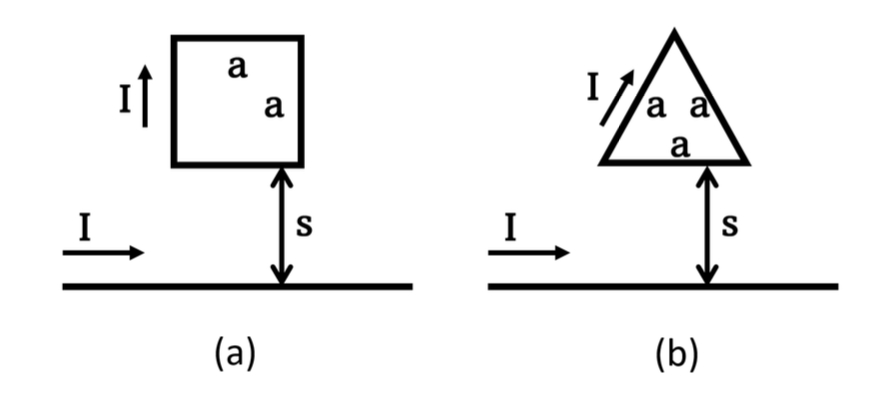
\includegraphics[scale = 0.5]{oz03/resources/Oz3Oef1.png}
\end{center}

% \begin{description}[labelwidth=1.5cm, leftmargin=!]
%     \item[Geg. :]   
%     \item[Gevr. :]  
%     \item[Opl. :]  
% \end{description}

\begin{enumerate}[(a)]
    \item 
        \begin{description}[labelwidth=1.5cm, leftmargin=!]
            \item[Geg. :]   $I$,$s$,$a$
            \item[Gevr. :]  de lorentzkracht $F_L$
            \item[Opl. :]   De evenwijdige zijden zullen een kracht uitoefenen op de draad. We vinden: 
                            \begin{align*}
                                F_L &= F_{\parallel, s+a} - F_{\parallel, s} \\ 
                                    % &= \dfrac{\mu_0I^2a}{2\pi}\left( \dfrac{1}{s+a} -\dfrac{1}{s} \right) \\
                                    &= \dfrac{\mu_0I^2}{2\pi}\dfrac{a^2}{s(s+a)} \\
                                \intertext{ Vectorieel wordt dit:}
                                \Vec{F}_L &= \dfrac{\mu_0I^2}{2\pi} \dfrac{a^2}{s(s+a)}(-\hat{j})
                            \end{align*}
        \end{description}
    \item 
        \begin{description}[labelwidth=1.5cm, leftmargin=!]
            \item[Geg. :]   $I$,$s$,$a$
            \item[Gevr. :]  de lorentzkracht $F_L$
            \item[Opl. :]   We berekenen eerst de infinitesimale kracht veroorzaakt door de schuine draden: 
                            \begin{equation*}
                                dF_{\text{schuin}} = \dfrac{\mu_0I^2\sin(60^\circ)}{2\pi}\dfrac{1}{r}dr
                            \end{equation*}
                            Hierover integreren we: 
                            \begin{align*}
                                F_{\text{schuin}} &= \int dF_{\text{schuin}} \\
                                                  &= \dfrac{\mu_0I^2}{2\pi\sin(60^\circ)} \int_s^{s+a\sin(60^\circ)} \tfrac{1}{r}dr \\
                                                  &= \dfrac{\mu_0I^2}{2\pi\sin(60^\circ)}\left(\ln(\tfrac{s+a\sin(60^\circ)}{s}) \right)
                            \end{align*}
                            Via superpositie vinden we: 
                            \begin{align*}
                                F_L &= 2F_{\text{schuin}} - F_{\parallel, s} \\
                                    &= \dfrac{\mu_0I^2}{2\pi}\left(\tfrac{1}{\sin(60^\circ)}\ln(\tfrac{s+a\sin(60^\circ)}{s}) - \dfrac{a}{s}\right)
                            \end{align*}
                            Vectorieel wordt dit:
                            \begin{equation*}
                                \Vec{F}_L = \dfrac{\mu_0I^2}{2\pi}\left( \tfrac{a}{s} - \tfrac{1}{\sin(60^\circ)}\left(\ln(\tfrac{s+a\sin(60^\circ)}{s}) \right) \right) (-\hat{j})
                            \end{equation*}
        \end{description}
        
\end{enumerate}

\vspace{1cm}